\documentclass[a4paper,11pt]{style-esi/td}

\usepackage{style-esi/licence}
\usepackage{style-esi/exercice}
\usepackage{style-esi/listing}
\usepackage{style-esi/tutoriel}
\usepackage{style/dev1}
\usepackage{amsmath}
\usepackage{amssymb}
\usepackage{placeins}

\begin{document}

\seance{12}{Mise en pratique : Le mot le plus long}{td12-mot-le-plus-long}{
	Dans ce TD vous utiliserez les notions vues précédemment 
	afin de réaliser le jeu \og~le mot le plus long\fg. 

	\begin{center}
		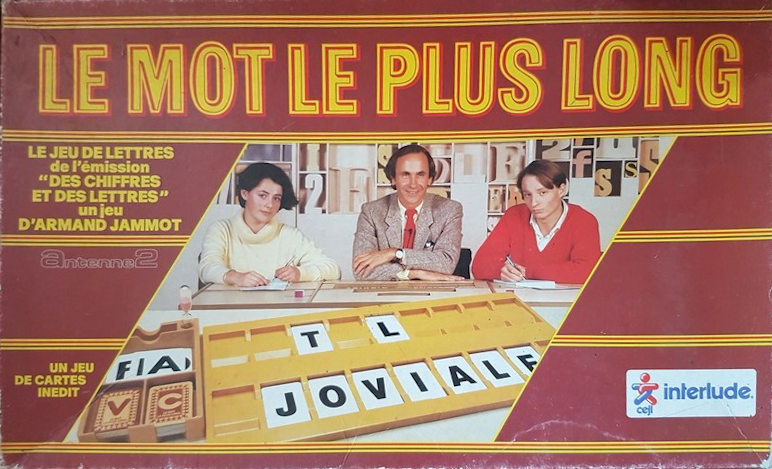
\includegraphics[width=13cm]{resources/lemotlepluslong}
	\end{center}

}


\section{Le mot le plus long}

	Le mot le plus long est un jeu de lettres à deux joueurs qui se déroule en
	plusieurs manches. Le nombre de manches est choisi au départ, par exemple 5 manches.
	Une manche se déroule en 2 étapes. 

	
	Tout d'abord les joueurs, chacun à leur tour, 
	tirent au hasard soit une voyelle, soit une consonne (le joueur choisit), 
	jusqu'à obtenir 9 lettres. À chaque fois qu'une lettre est tirée 
	(voyelle ou consonne), la lettre est dévoilée aux joueurs afin qu'ils puissent
	continuer en connaissance de cause.

	Ensuite les joueurs cherchent le mot le plus long avec les lettres disponibles.
	Chaque joueur annonce la longueur du mot trouvé. Celui qui a trouvé le mot le 
	plus long le forme avec les lettres disponibles. On vérifie alors que c'est 
	bien un mot du dictionnaire. Le joueur gagne autant de points que le nombre
	de lettres de son mot. 
			
	Nous allons vous guider tout au long de ce TD 
	afin de développer les différentes méthodes nécessaires 
	pour une version simplifiée à un seul joueur de ce jeu.


	Tout d'abord,
	créez une classe \mbox{LeMotLePlusLong} que vous placez dans le package \texttt{g12345.dev1.lemotlepluslong}.
	Créez aussi la méthode principale qui, dans un premier temps, 
	affiche un message de bienvenue au 'mot le plus long'.

 	\begin{Exercice}{Hasard}
		\'Ecrivez la méthode \code{java}{int tirerHasard(int min, int max)} qui
		retourne un nombre au hasard compris entre \texttt{min} et
		\texttt{max} reçus en paramètre.
		
		Par exemple si la méthode reçoit 3 et 8, elle retourne 6.
		
		Astuce: utilisez la méthode \texttt{random} de la classe \texttt{Math} qui 
		retourne un nombre réel entre 0 (compris) et 1 (non-compris).
	\end{Exercice} 

 
 	\begin{Exercice}{Voyelle}
		\'Ecrivez la méthode \code{java}{char tirerVoyelle()} qui retourne une voyelle 
		tirée au hasard.
		
		Cette méthode fera un appel à la méthode \texttt{tirerHasard} 
		de l'exercice précédent.
	\end{Exercice} 

 	\begin{Exercice}{Consonne}
		\'Ecrivez la méthode \code{java}{char tirerConsonne()} qui retourne une consonne 
		tirée au hasard.
	\end{Exercice} 

 	\begin{Exercice}{Afficher les lettres}
 		\'Ecrivez la méthode \code{java}{void afficherLettres(char[] lettres)}
		qui affiche le contenu du tableau \texttt{lettres}.
		
		Par exemple si la méthode reçoit le tableau 
                \begin{quote}\ttfamily
		\{'E', 'E', 'I', 'O', 'C', 'D', 'M', 'R', 'Z'\},
              \end{quote}
		elle doit afficher~:
		\begin{quote}\ttfamily
		E E I O C D M R Z
		\end{quote}
		
		Cette méthode permettra d'afficher les lettres tirées par les joueurs.
	\end{Exercice} 

 	\begin{Exercice}{Demander les lettres}
		\'Ecrivez la méthode \code{java}{char[] demanderLettres()}
		qui demande à l'utilisateur s'il veut une voyelle ou une consonne
		et qui, en fonction de la réponse, tire une voyelle ou une consonne.
		La méthode affiche les lettres déjà tirées et répète la demande
		et le tirage 9 fois.
		 
		La méthode retourne un tableau de 9 caractères contenant les lettres tirées. 
		
		Intégrez cela dans la méthode principale, c'est-à-dire, ajoutez un appel à 
		la méthode \texttt{demanderLettres} dans la méthode principale.
	\end{Exercice} 

	
 	\begin{Exercice}{Demander un mot}
		\'Ecrivez la méthode \code{java}{String demanderMot()}
		qui demande à l'utilisateur le mot le plus long qu'il a trouvé.
		 
		La méthode retourne le mot donné par l'utilisateur. 
		
		Intégrez cela dans la méthode principale.
	\end{Exercice} 
	
 	\begin{Exercice}{Vérifier les lettres}
 			\'Ecrivez la méthode 
 			\code{java}{boolean vérifierLettres(char[] lettres, String mot)}
		qui vérifie que le mot proposé est possible avec les lettres 
		disponibles. 
		
		Attention: vous ne pouvez pas modifier le tableau \texttt{lettres}.
		
		Astuce: vous pouvez utiliser un tableau de travail, par exemple un 
		tableau de booléens qui indiquera si une lettre à déjà été utilisée.
		
		Cette méthode n'est pas triviale, elle doit être validée par des tests.
		Ajoutez des tests JUnit en prenant soin de tester les cas particuliers: 
		utilisation de la même lettre mais disponible une seule fois, utilisation de la 
		même lettre disponible plusieurs fois, utilisation d'une lettre non 
		disponible, etc.
		
		Complétez la méthode principale.
	\end{Exercice} 
	
 	\begin{Exercice}{Mot du dictionnaire}
 	 			\'Ecrivez la méthode 
 			\code{java}{boolean dansDictionnaire(String mot)}
		qui vérifie que le mot proposé se trouve dans le dictionnaire.
				
		Pour réaliser cet exercice, nous vous fournissons une librairie qui contient 
		un dictionnaire, ou plus exactement la liste de tous les mots
		acceptés par le jeu. Cette librairie vous est fournie : devez l'ajouter à votre projet sous forme de dépendance.
		 
                \begin{figure}[hb]\centering
                \includegraphics[height=6cm]{resources/whereIsPom}
                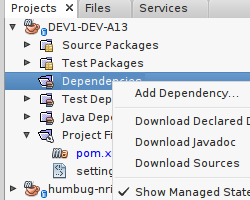
\includegraphics[height=6cm]{resources/add-dependency-1}
                \caption{\label{pompompom}Le fichier pom.xml (à gauche), et le menu pour ajouter une dépendance (à droite)}
              \end{figure}

                  \begin{figure}[hb]
                    \centering
                    \begin{Code}[basicstyle=\ttfamily]{xml}% ttfamily has the added benefit of not turning the hyphen (-) into a MINUS SIGN (−). See also https://tex.stackexchange.com/questions/33185/listings-package-changes-hyphens-to-minus-signs
                    <repositories>
                        <repository>
                            <id>esi</id>
                            <name>esi</name>
                            <url>https://maven.esi-bru.be/</url>
                        </repository>
                    </repositories>
                  \end{Code}
                  \caption{Code à ajouter au fichier \texttt{pom.xml}}
                  \label{pomrepository}
                \end{figure}


                
		\begin{infoit}{Dépendances}	
		% \subsection*{Mais qu’est-ce qu’un jar ?}
		% 	Un JAR (Java Archive) est un fichier Zip utilisé pour distribuer un 
		% 	ensemble de classes Java. Ce format est utilisé pour stocker les 
		% 	définitions des classes, ainsi que des méta-données, constituant 
		% 	l’ensemble d’un programme. [Wikipedia]
		
                \subsection*{Qu'est-ce qu'une dépendance ?}
                Un \emph{dépendance} est du code dont votre projet \emph{dépend}.
                Votre projet va \emph{dépendre} du dictionnaire pour son fonctionnement.
                L'idée de dépendance est comprise par l'outil Maven via le fichier pom.xml.
                % Pour que Maven cherche et trouve les dépendances, il faut
                % \begin{enumerate}
                % \item lui indiquer des \emph{repositories} (dépôts) où chercher, et
                % \item \emph{déclarer} la dépendance.
                % \end{enumerate}
                
		% \subsection*{Comment ajouter un jar donné ?}
		% 	Sous Netbeans, pour pouvoir utiliser les classes d’un .jar donné, il suffit :
		% 	\begin{enumerate}
		% 		\item de copier ce .jar dans un sous-dossier de votre projet (par exemple
		% 			dans le dossier lib, que vous créez pour l’occasion).
		% 		\item d’ajouter ce .jar aux librairies de votre projet.
		% 	\end{enumerate}

                \medskip
                \subsection*{Le fichier pom.xml ?}
                C'est un fichier de configuration de Maven.
                Vous le trouverez dans Netbeans sous \emph{Project Files} (voir figure~\vref{pompompom}, à gauche).
                Prenez quelques secondes pour essayer de comprendre le format de ce fichier : c'est un fichier XML%
                \footnote{
                  des balises qui s'ouvrent, possèdent (parfois) des attributs,
                  ont du contenu, et se ferment.
                  \texttt{<balise attribut="valeur">contenu</balise>}
                  En outre, l'indentation permet de visualiser le fait que certaines balises sont "contenues" dans d'autres.
                }.

                \medskip
                \subsection*{Ajouter la dépendance}
                \begin{enumerate}
              \item Ajoutez d'abord le dépôt des librairies de l'ESI en ajoutant le code de la figure~\vref{pomrepository} dans la balise \texttt{project} (par exemple juste avant la ligne \texttt{</project>}).
                Vérifiez que Netbeans ne souligne rien en rouge, puis sauvez.

                
              \item Ensuite, après un clic droit sur Dependencies, cliquez sur Add dependency (voir figure~\vref{pompompom}, à droite).
                Une fenêtre s'ouvre.
                Dans Query, indiquez \emph{Dictionnaire} et appuyez sur Enter.
                Rapidement, le résultat suivant doit s'afficher ; sélectionnez-le et confirmez :
                \begin{center}
                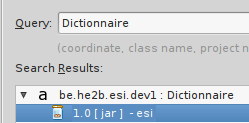
\includegraphics[scale=0.6]{resources/add-dependency-2}
                \end{center}
                C'est fait ! Re-lancez votre projet pour vérifier qu'aucune erreur n'est apparue.

              \end{enumerate}
              \end{infoit}

              	Une fois la dépendance ajoutée à votre projet, comment l'utiliser ?
			La librairie que nous vous fournissons contient une seule classe : 
			la classe \texttt{Dictionnaire} qui se trouve dans le package 
			\texttt{esi.dev1.util}. Cette classe possède une méthode 
			\code{java}{String[] mots()} qui retourne un tableau contenant tous les mots
			du dictionnaire. Pour l'utiliser il suffit donc d'appeler cette méthode
			et de récupérer une référence vers ce tableau de mots:
			
			\code{java}{String[] dico = Dictionnaire.mots();}	
			
			Vous avez maintenant un tableau contenant tous les mots du dictionnaire.
			Par exemple \code{java}{System.out.println(dico[58]);} affichera 
			le 59\ieme{} mot de ce dictionnaire.
	\end{Exercice} 
        \FloatBarrier
 	\begin{Exercice}{Le meilleur mot}
 	 	\'Ecrivez la méthode 
 		\code{java}{String meilleurMot(char[] lettres)}
		qui parcourt le dictionnaire à la recherche du mot le plus long faisable 
		avec les lettres disponibles. 
		Si plusieurs mots sont possibles on en choisit ici un seul.

		Testez votre méthode avec plusieurs tests JUnit.

                Intégrez cela dans la méthode principale.
	\end{Exercice}

 	\begin{Exercice}{Bonus 1 - Les meilleurs mots}
 	 	\'Ecrivez la méthode 
 		\code{java}{String[] meilleursMots(char[] lettres)}
		qui retourne la liste de tous les mots les plus longs du dictionnaire 
		faisables avec les lettres disponibles.

		Testez votre méthode avec plusieurs tests JUnit.

		Intégrez cela dans la méthode principale.
	\end{Exercice}


 	\begin{Exercice}{Bonus 2 - 2 joueurs}
		Développez le jeu à plusieurs manches, avec 2 joueurs, 
		ainsi que la gestion du score et du gagnant.
		Pour cela vous pouvez vous référer aux règles officielles  
		disponibles sur internet\footnote{Par exemple~:\url{https://www.trictrac.net/jeu-de-societe/le-mot-le-plus-long-3/details}}.
	\end{Exercice}
		
 	\begin{Exercice}{Bonus 3 - Fréquence des lettres}
		
		Pour que le jeu soit agréable il faudrait que la fréquence des
		différentes lettres ne soit pas uniforme. En d'autres mots, il est
		préférable d'avoir plus souvent un 'e' ou un 'a' qu'un 'y', un 's'
		ou un 'z'. Modifiez vos méthodes \texttt{voyelle} et \texttt{consonne}
		afin d'ajuster la probabilité des différentes lettres. 
		
		Vous pouvez vous baser par exemple sur la fréquence des lettres en français:
		 \url{https://fr.wikipedia.org/wiki/Fr%C3%A9quence_d%27apparition_des_lettres_en_fran%C3%A7ais}
	
	 \end{Exercice}
		


\end{document}

%%% Local Variables:
%%% TeX-master: t
%%% End:
